\documentclass[11pt,a4paper]{article}
\usepackage[utf8]{inputenc}
\usepackage[T1]{fontenc}
\usepackage[english]{babel}

\title{
	Computer Exercise 1\\
	EL2520 Control Theory and Practice
}
\author{
	Sifan Jiang\\
	sifanj@kth.se\\
	961220-8232
	\and
	Jiaqi Li\\
	jiaqli@kth.se\\
	960326-1711
}

\newcommand{\image}[3]{
	\begin{figure}[!ht]
		\centering
	    \includegraphics[width=#1\textwidth]{#2}
		\caption{#3}
		\label{fig:#2}
	\end{figure}
}

% My packages
\usepackage{algorithm, algorithmic, listings} % Code
\usepackage{amsmath, amstext, amssymb, amsfonts, amsthm, dsfont, cancel, gensymb, mathtools, textcomp} % Math
\usepackage{color, xcolor} % Color
\usepackage{diagbox, tabularx} % Table
\usepackage{enumerate} % List
\usepackage{epsfig, epstopdf, graphicx, multicol, multirow, palatino, pgfplots, subcaption, tikz} % Image.
\usepackage{fancybox}
\usepackage{verbatim}


\usepackage[font=footnotesize]{caption} % labelfont=bf
\usepackage[font=scriptsize]{subcaption} % labelfont=bf
\usepackage[margin=1in]{geometry}
\usepackage[hidelinks]{hyperref}
\epstopdfsetup{outdir=./Figure/Converted/}
\graphicspath{{./Figure/}}

\makeatletter
\def\input@path{{./Figure/}}
\makeatother

\pgfplotsset{compat=1.13}

\begin{document}
\maketitle

% Minimum phase case
\section*{Minimum phase case}
\par The controller is given by
\begin{align*}
	F(s) = \begin{bmatrix}
		1.6776(1+\dfrac{1}{5.904s}) & 0 \\
		0 & 2.0137(1+\dfrac{1}{6.391s})
	\end{bmatrix}		
\end{align*}
\begin{figure}[!ht]
	\footnotesize
	\centering 
	\begin{subfigure}[t]{.495\linewidth}
		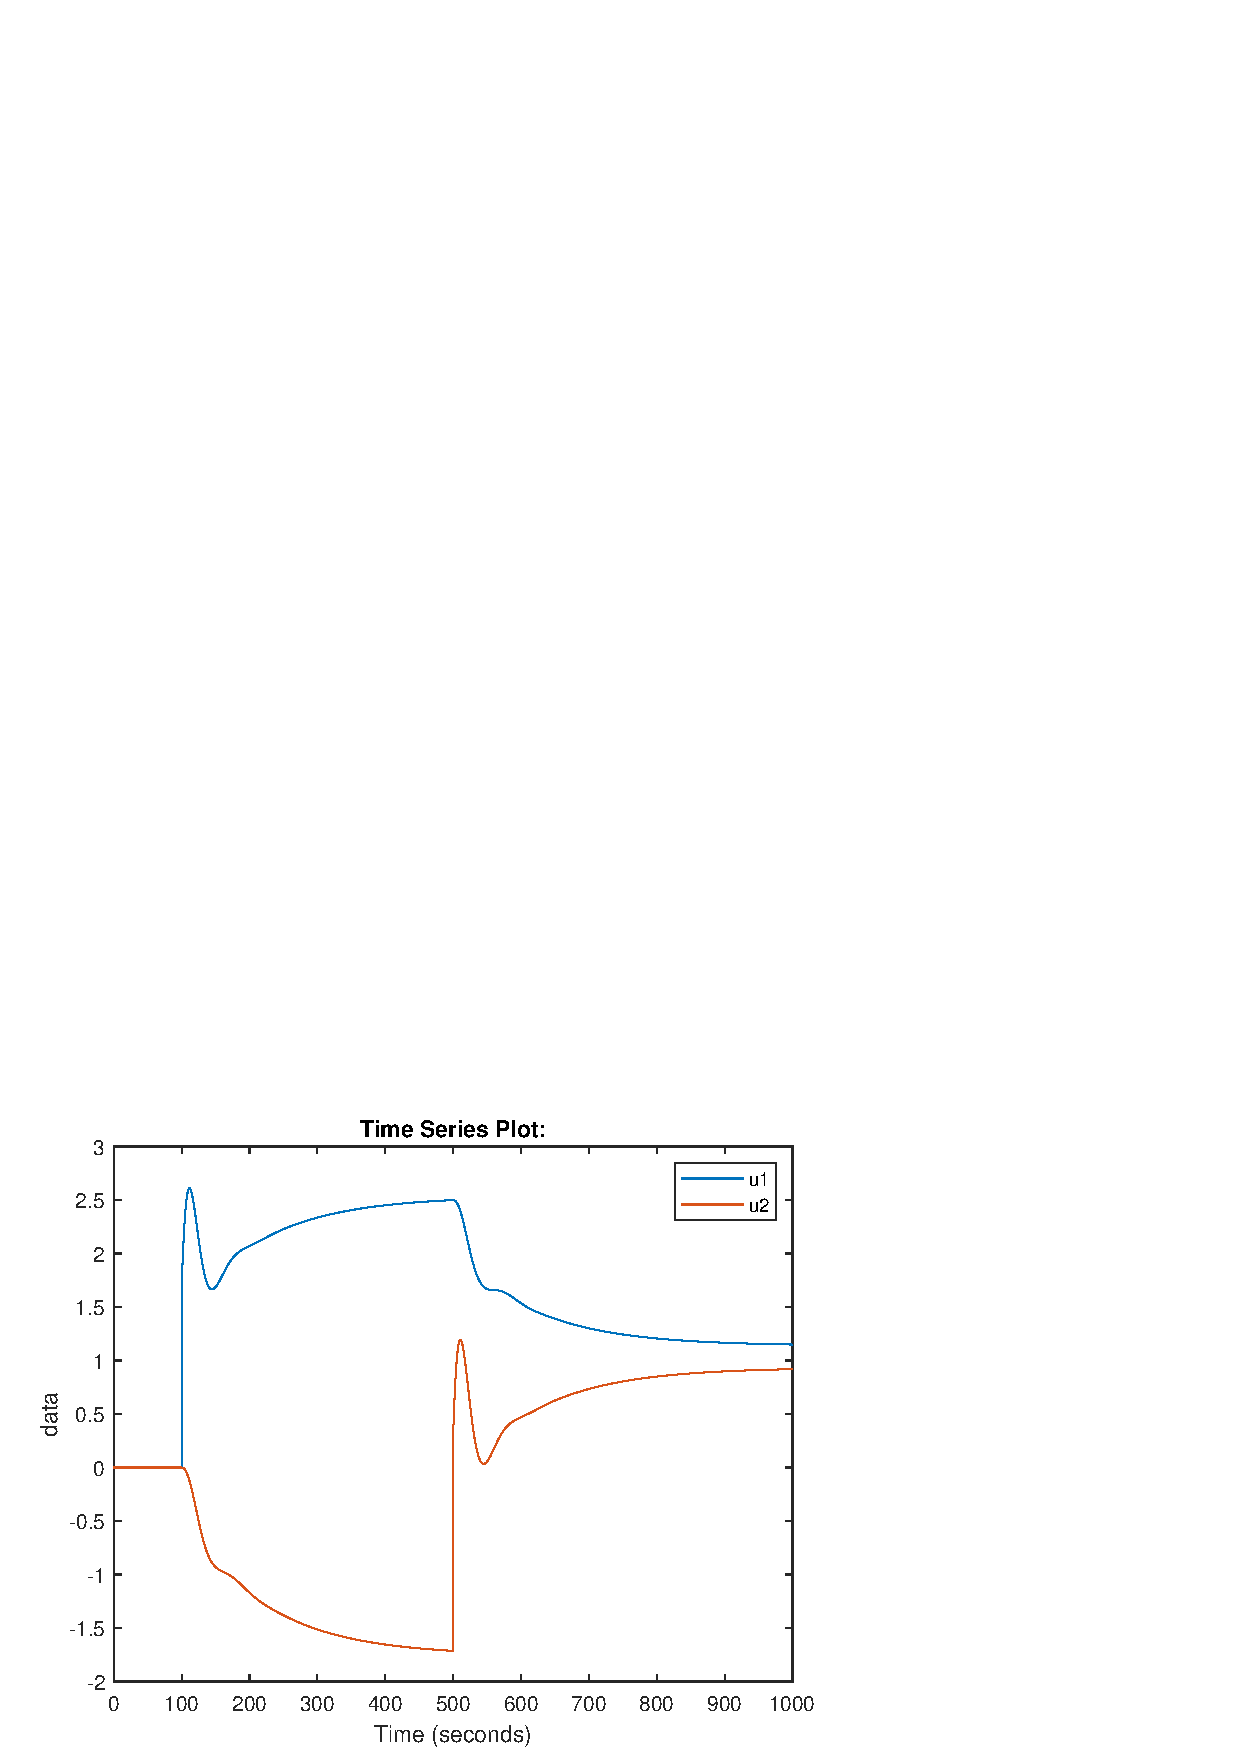
\includegraphics[width=\columnwidth]{3231}
		\caption{Response of the control signal $u$.}
		\label{fig:3231}
	\end{subfigure}
	\begin{subfigure}[t]{.495\linewidth}
		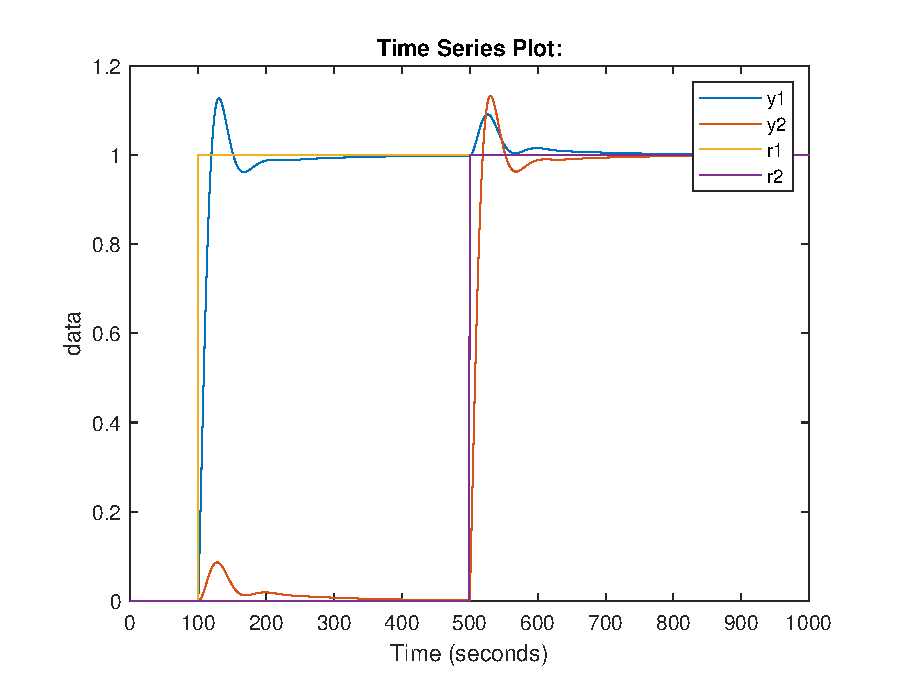
\includegraphics[width=\columnwidth]{3232}
		\caption{Response of the output $y$ with the reference $r$.}
		\label{fig:3232}
	\end{subfigure}
	\caption{Simulink plots from exercise 3.2.3.}
	\label{fig:MPSimulink}
\end{figure}
\begin{figure}[!ht]
	\footnotesize
	\centering 
	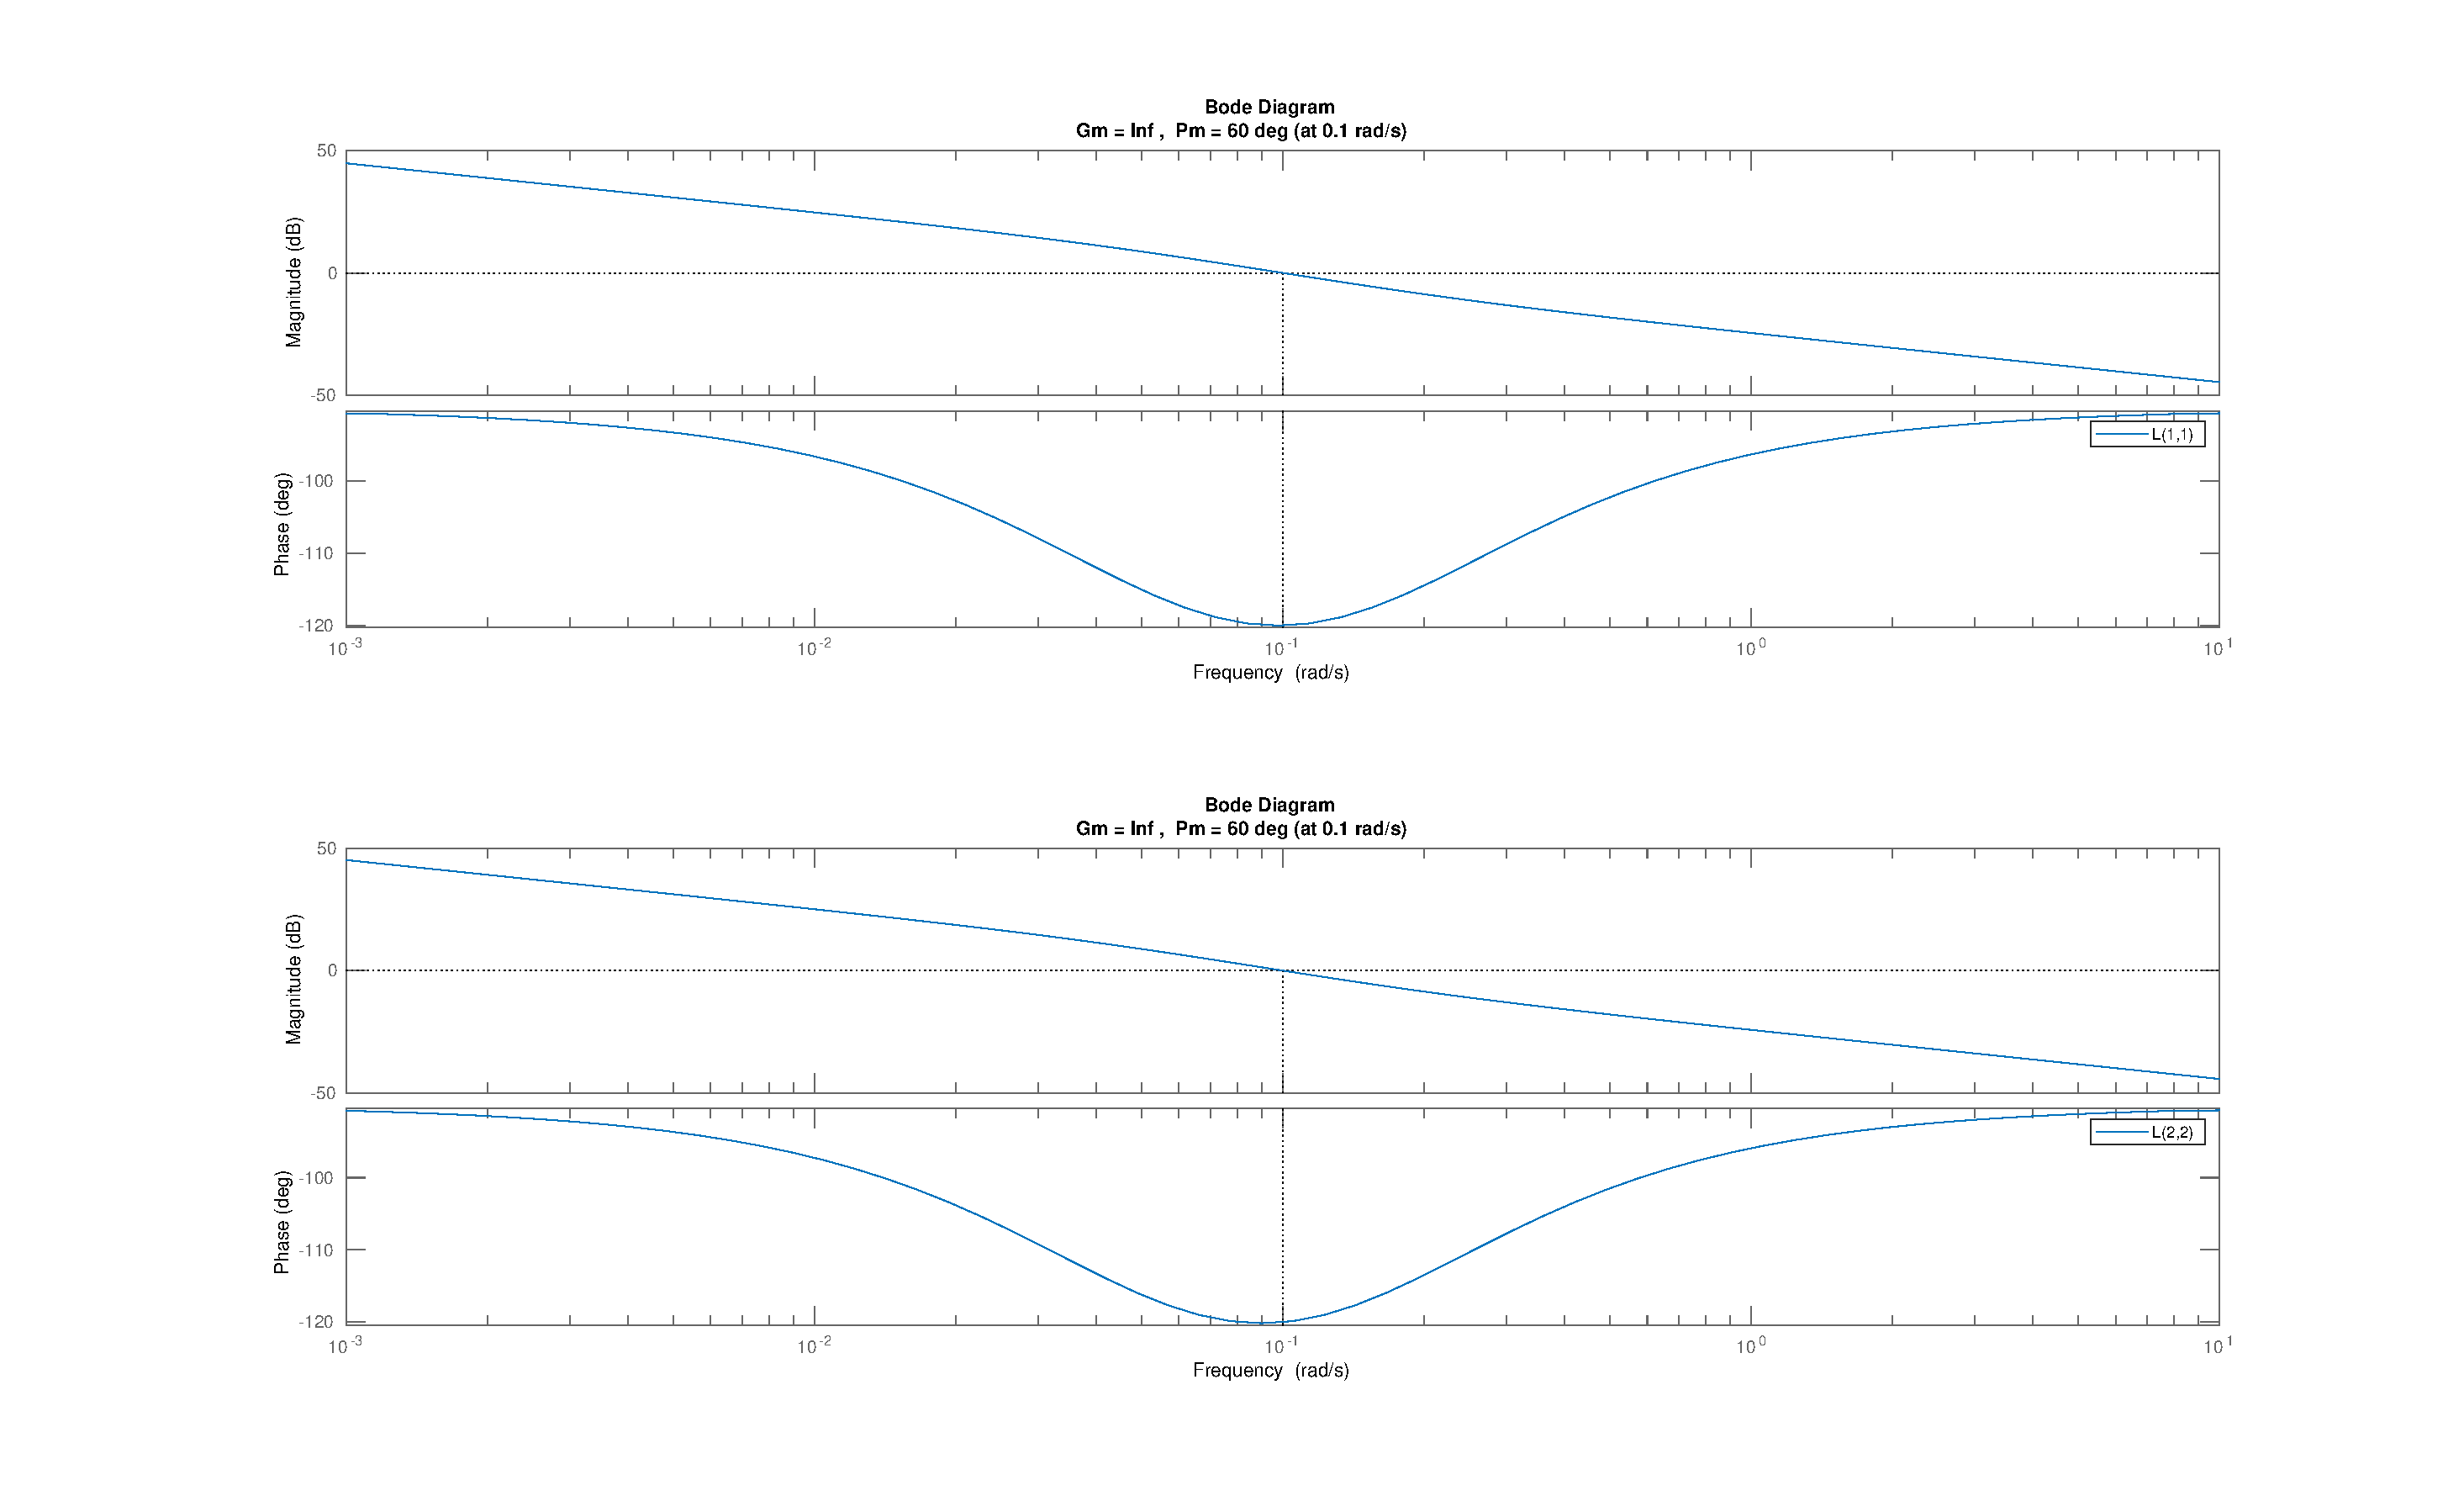
\includegraphics[width=\textwidth]{321}
	\caption{Bode diagram of the loop gain $L(s)$ from exercise 3.2.1.}
	\label{fig:MPBodeL}
\end{figure}

\par From fig~\ref{fig:3232}, we can conclude that the two outputs are coupled but not strongly coupled, since both of the inputs, $r_{1}$ and $r_{2}$ would affect both outputs. However, $r_{1}$ can have much obvious effect on $y_{1}$ and $r_{2}$ can have much obvious effect on $y_{2}$. However, when $r_{1}$ comes, $y_{1}$ increases much more than $y_{2}$, and $y_{2}$ recover to its original state after a while, which is similar for the case of $r_{2}$. Thus, the pairing is satisfied. Also, as we can see, the overshooting is small enough.

\par From fig~\ref{fig:MPSingular}, which is the singular values of the $S$ and $T$ of the system, the singular values are both small when the frequency approaching the $\omega_{c}$, implying the controller is good. Also, we can learn that the controller will be more sensitive and less robust to the disturbance at low frequency, and less sensitive and more robust to the disturbance at high frequency.

\begin{figure}[!ht]
	\footnotesize
	\centering 
	\begin{subfigure}[t]{.495\linewidth}
		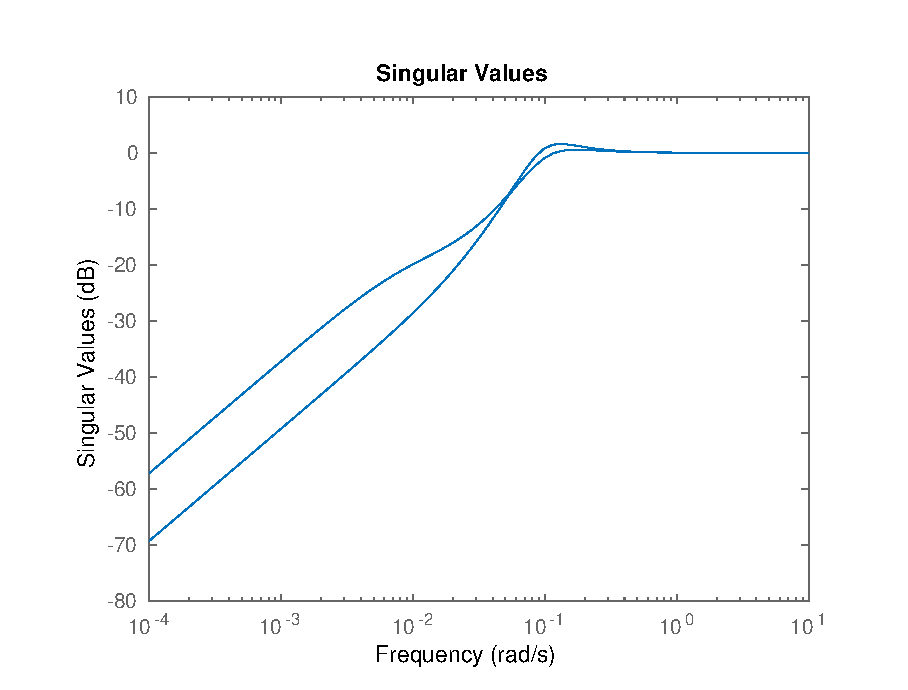
\includegraphics[width=\columnwidth]{322}
		\caption{Singular values of the sensitivity $S$.}
		\label{fig:322}
	\end{subfigure}
	\begin{subfigure}[t]{.495\linewidth}
		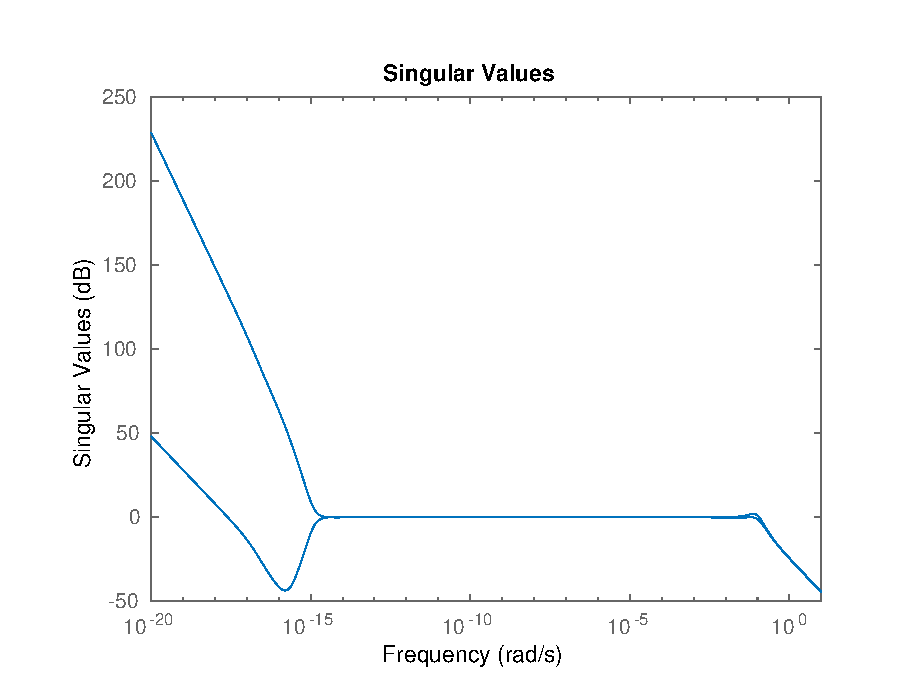
\includegraphics[width=\columnwidth]{3222}
		\caption{Singular values of the complementary sensitivity $T$.}
		\label{fig:3222}
	\end{subfigure}
	\caption{Singular values of $S$ and $T$.}
	\label{fig:MPSingular}
\end{figure}


% -------------------------------------------------- %
% Non-minimum phase case
\section*{Non-minimum phase case}
\par The controller is given by
\begin{align*}
	F(s) = \begin{bmatrix}
		0 & 0.1437(1+\dfrac{1}{4.8107s}) \\
		0.1469(1+\dfrac{1}{3.9426s}) & 0    	
    \end{bmatrix}
\end{align*}
\begin{figure}[!ht]
	\footnotesize
	\centering 
	\begin{subfigure}[t]{.495\linewidth}
		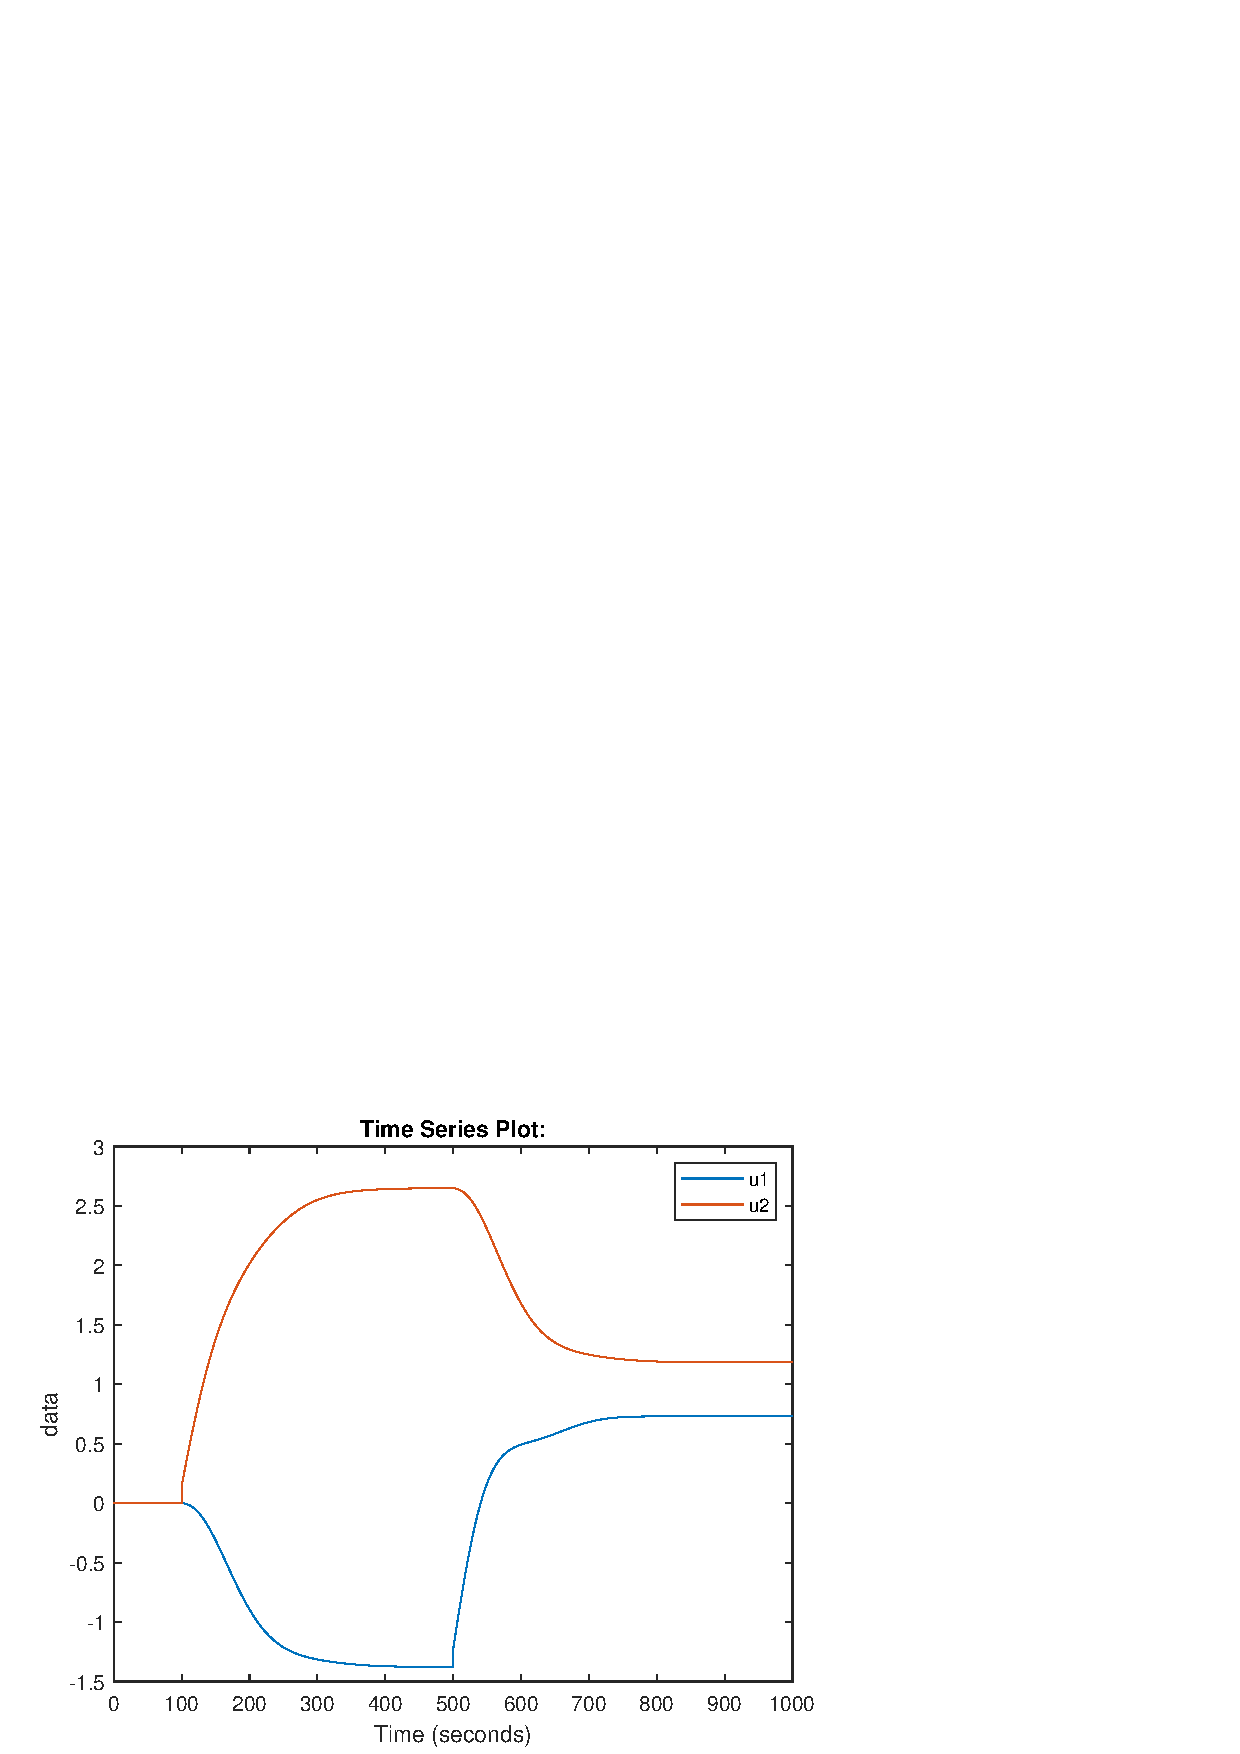
\includegraphics[width=\columnwidth]{3331}
		\caption{Response of the control signal $u$.}
		\label{fig:3331}
	\end{subfigure}
	\begin{subfigure}[t]{.495\linewidth}
		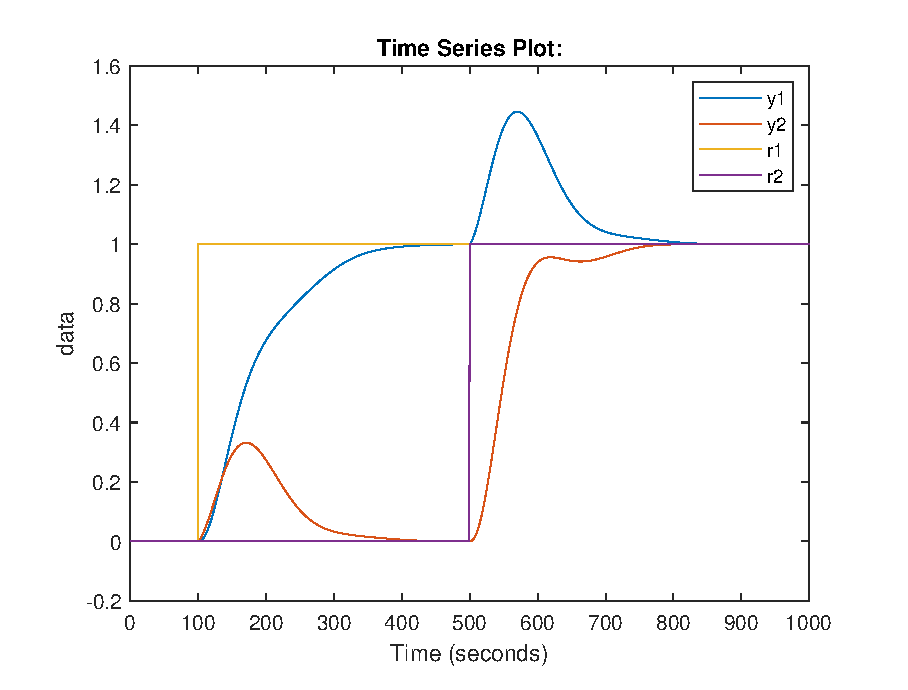
\includegraphics[width=\columnwidth]{3332}
		\caption{Response of the output $y$ with the reference $r$.}
		\label{fig:3332}
	\end{subfigure}
	\caption{Simulink plots from exercise 3.2.3.}
	\label{fig:NMPSimulink}
\end{figure}
\begin{figure}[!ht]
	\footnotesize
	\centering 
	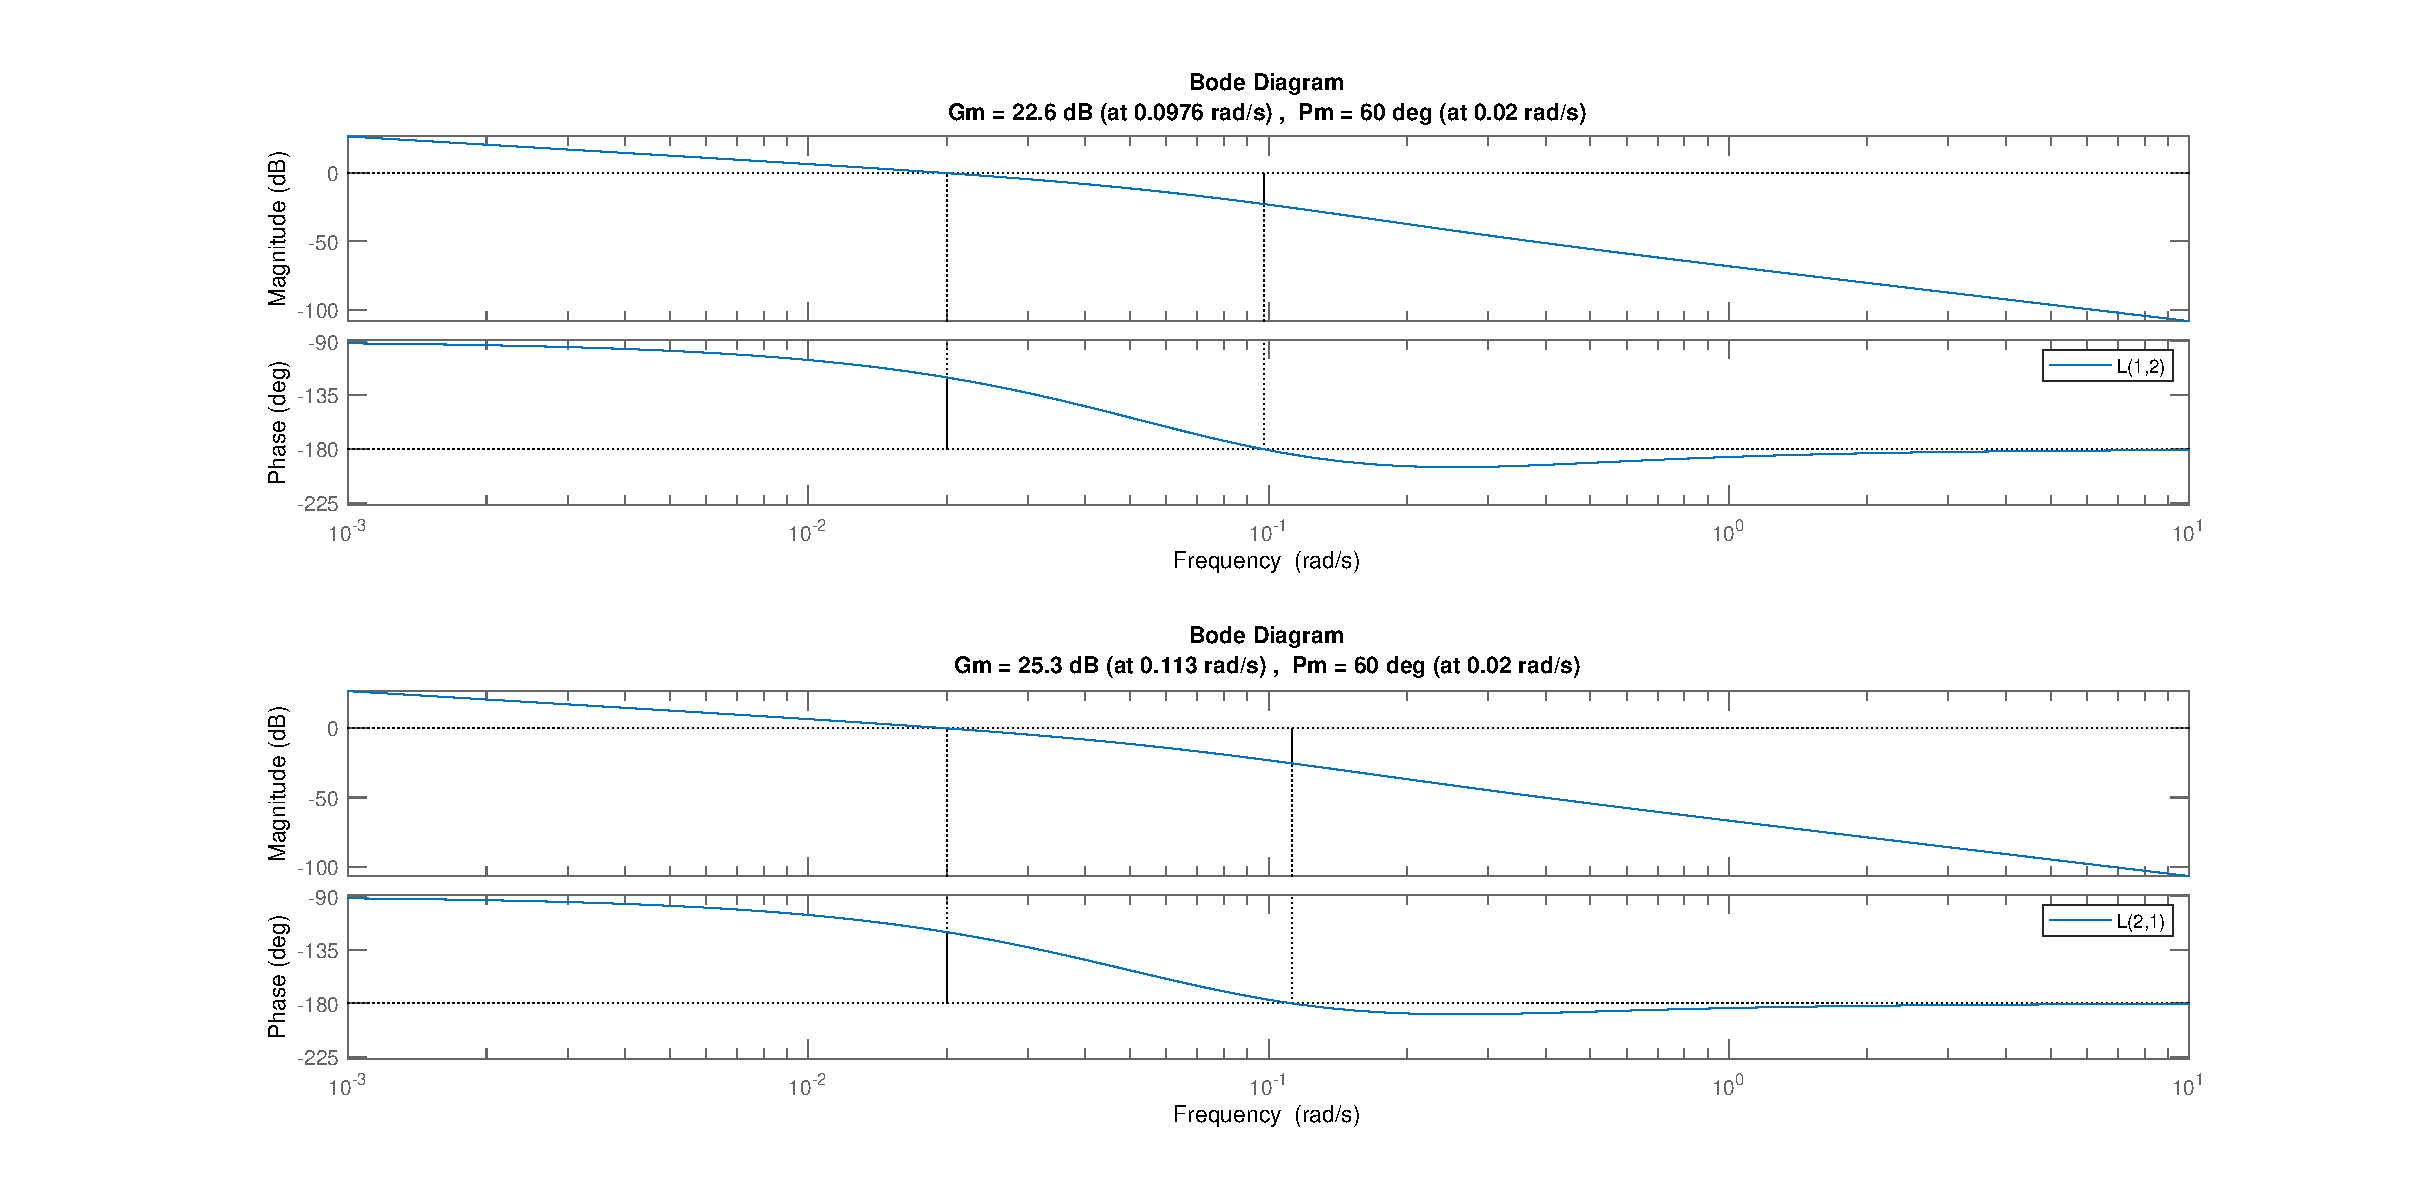
\includegraphics[width=\textwidth]{331}
	\caption{Bode diagram of the loop gain $L(s)$ from exercise 3.2.1.}
	\label{fig:NMPBodeL}
\end{figure}

\par The singular values of the sensitivity and complementary sensentivity are shown in the fig~\ref{fig:3321} and \ref{fig:3322}. As we see, the controller will be more sensitive and less robust to the disturbance at low frequency, and less sensitive and more robust to the disturbance at high frequency.

\par As shown in the fig~\ref{fig:NMPSimulink}, the outputs are coupled and it is still strongly coupled. When given a step response, the unrelated output will gain more impulse than minimum phase case, but it needs more time to be steady again. So we can conclude that the controller is not good enough.

\begin{figure}[!ht]
	\footnotesize
	\centering 
	\begin{subfigure}[t]{.495\linewidth}
		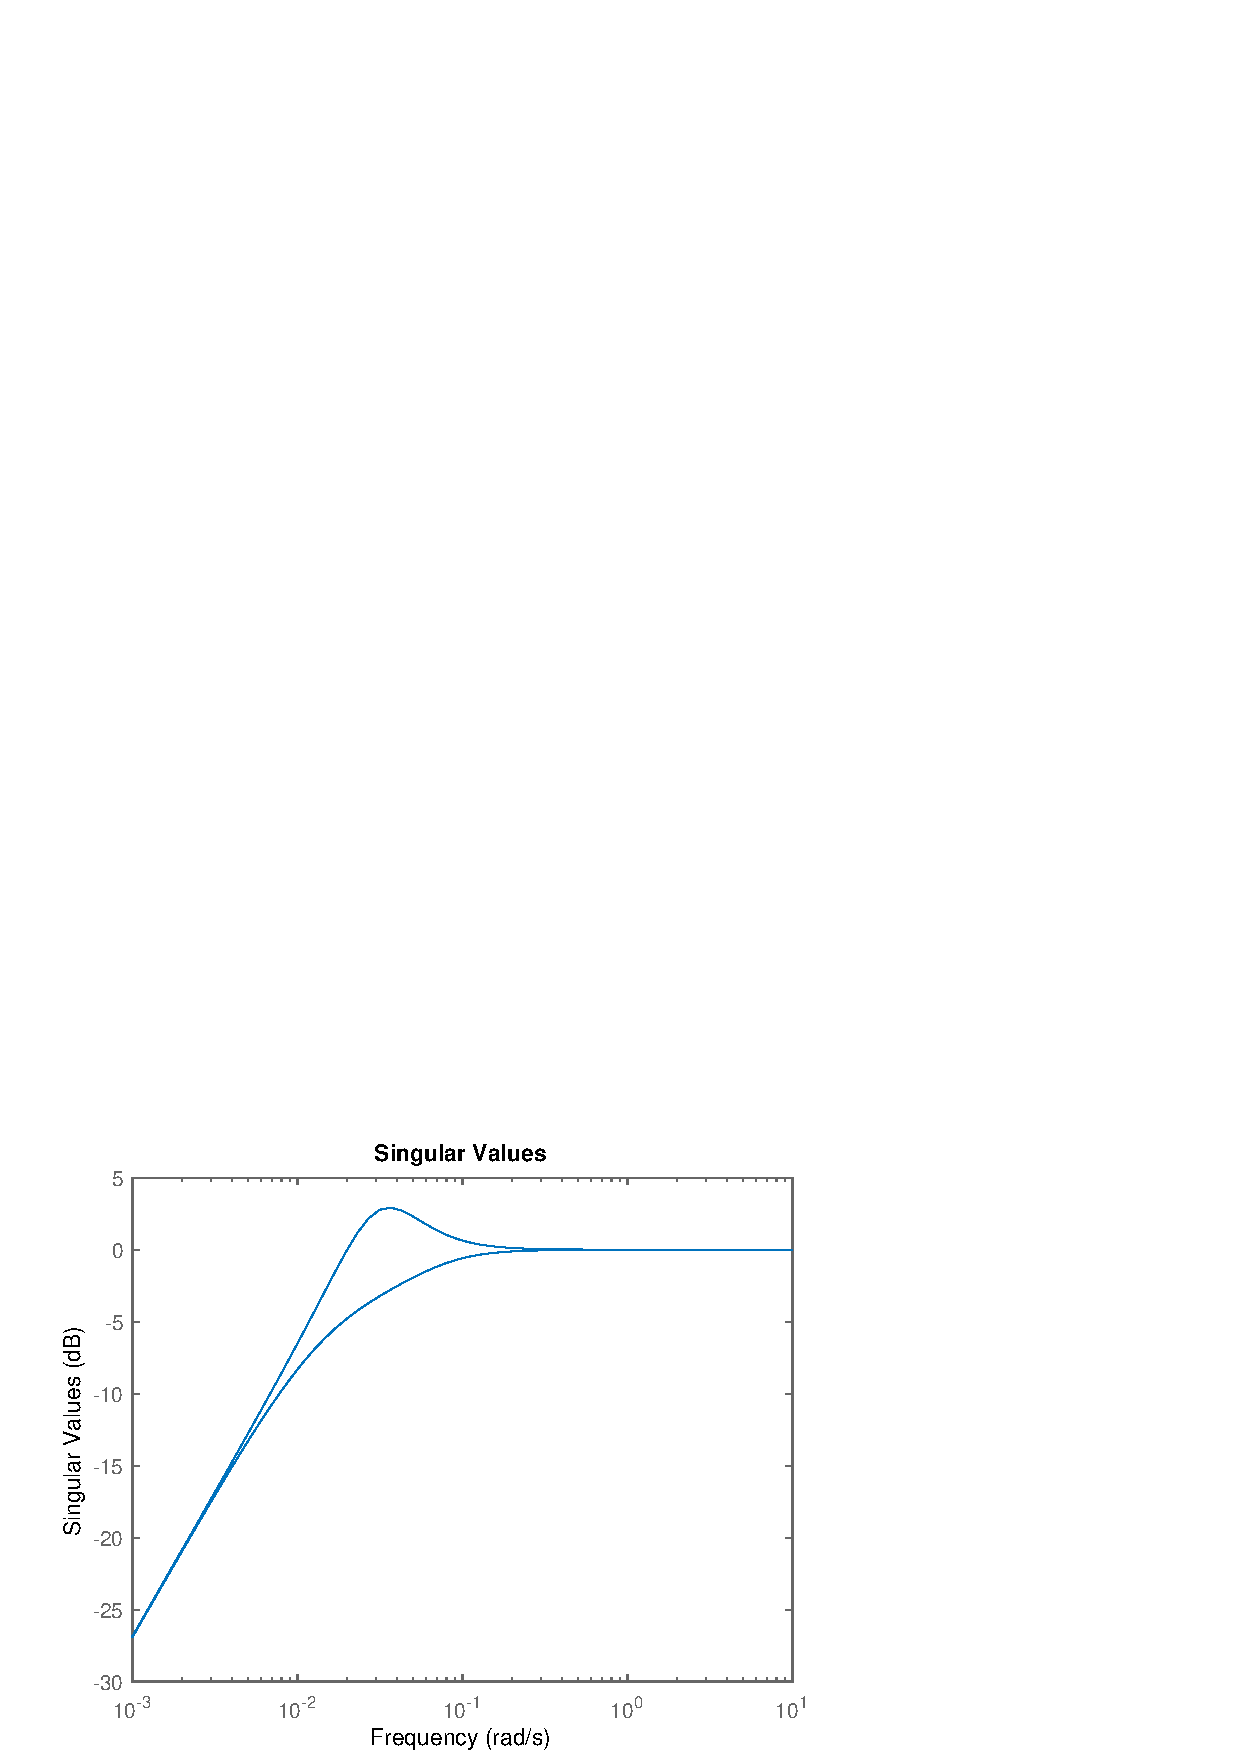
\includegraphics[width=\columnwidth]{3321}
		\caption{Singular values of sensitivity $S$.}
		\label{fig:3321}
	\end{subfigure}
	\begin{subfigure}[t]{.495\linewidth}
		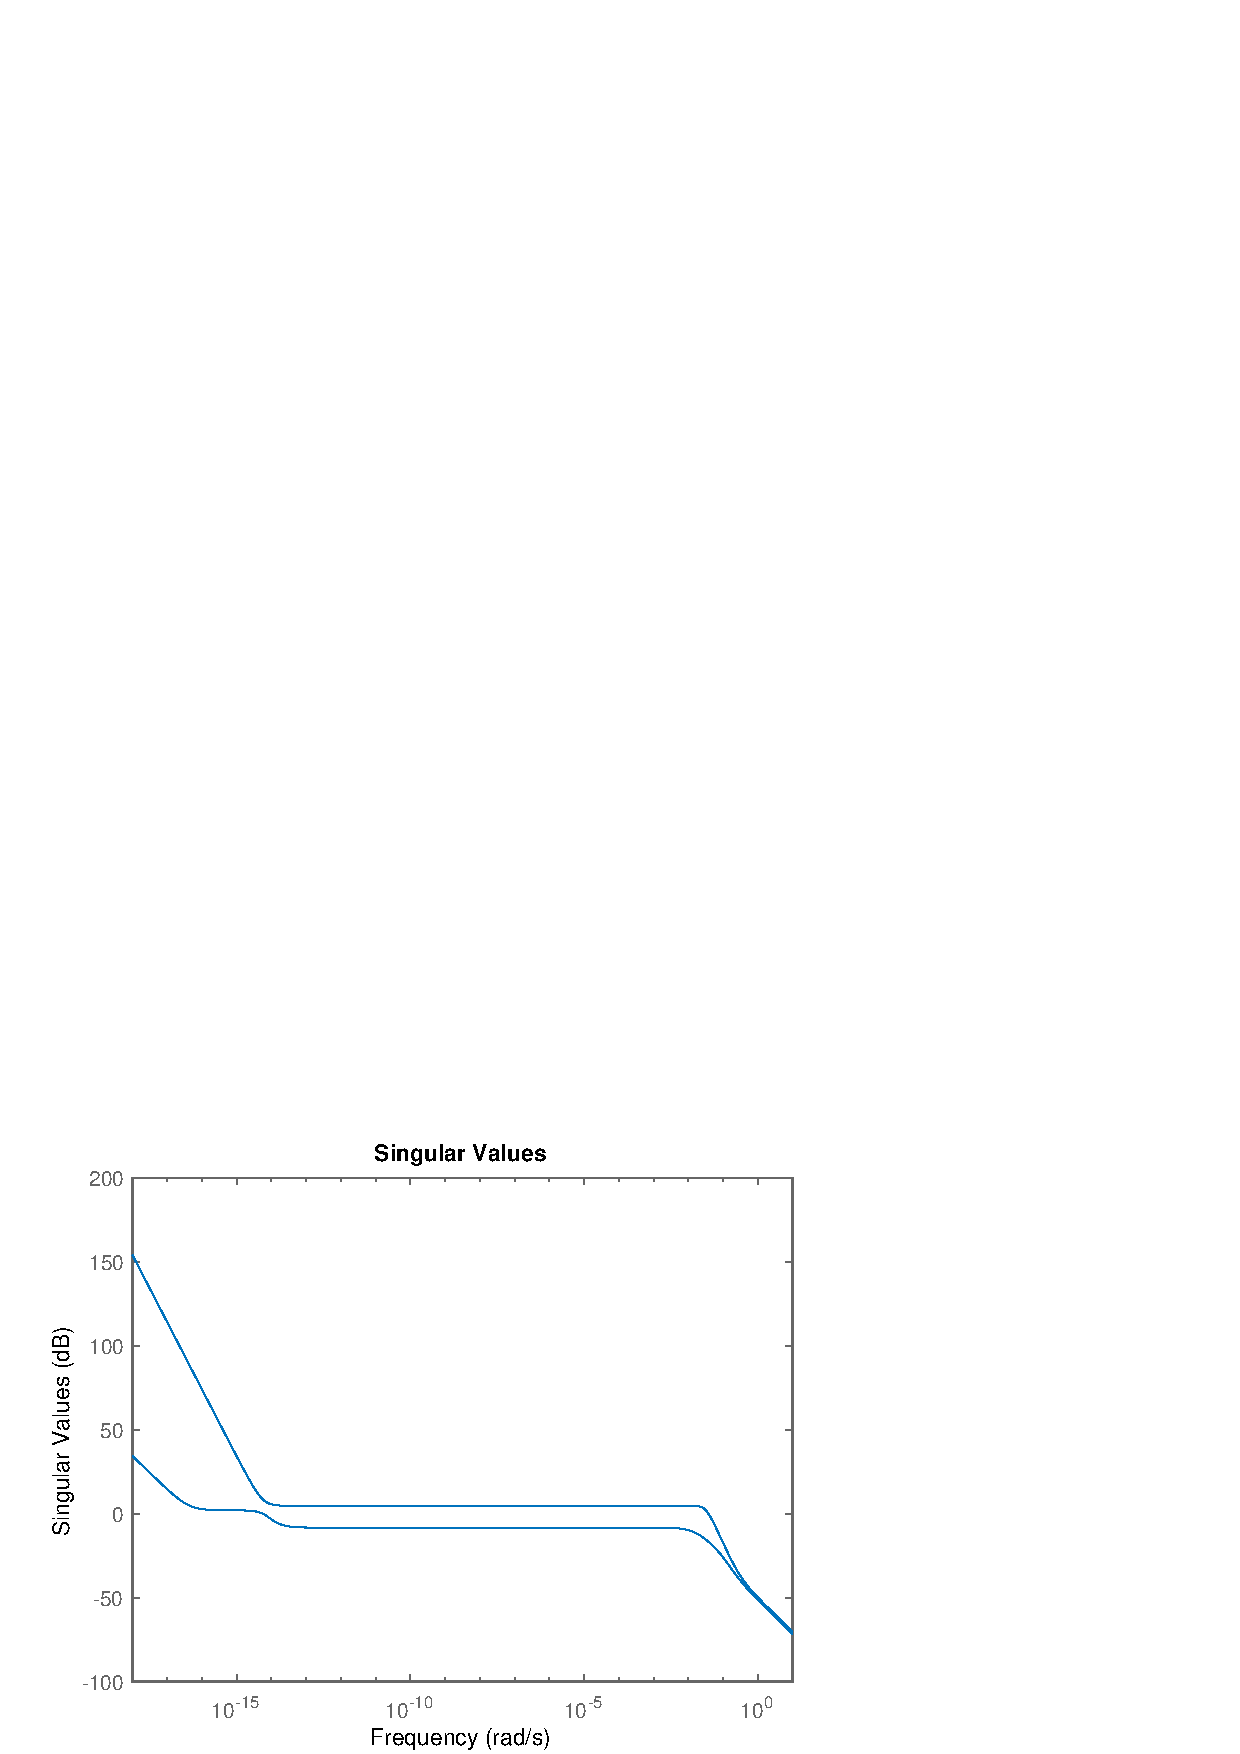
\includegraphics[width=\columnwidth]{3322}
		\caption{Singular values of complementary sensitivity $T$.}
		\label{fig:3322}
	\end{subfigure}
	\caption{Singular values of $S$ and $T$.}
	\label{fig:NMPSingular}
\end{figure}

\end{document}